\documentclass[11pt]{article}
\usepackage{amsmath}
\usepackage{amssymb}
\usepackage{graphicx}
\usepackage{tabularx}
\usepackage{fancyhdr}
\usepackage{lastpage}

% Page layout
\usepackage[top=1in, bottom=1in, left=1in, right=1in]{geometry}

% Header and footer
\pagestyle{fancy}
\fancyhf{}
\rfoot{Page \thepage}
\renewcommand{\headrulewidth}{0pt}

% Modified Question command with left-aligned number
\newcommand{\questiona}[2]{
    \noindent\textbf{Q#2.} #1 \hfill \textbf{[1 Mark]}
}

\newcommand{\questionb}[2]{
    \noindent\textbf{Q#2.} #1 \hfill \textbf{[2 Marks]}
}

\begin{document}

% Title section with horizontal line
\begin{center}
    \Large\textbf{GATE 2018 - Civil Engineering (CE)} \\
    \large\textbf{General Aptitude and Technical Questions} \\
    \rule{\textwidth}{0.5pt} % Horizontal line below heading
\end{center}

\vspace{0.5cm}

% General Aptitude Section
\section*{General Aptitude}

\questiona{"The driver applied the \_\_\_\_\_ as soon as she approached the hotel where she wanted to take a \_\_\_\_\_." The words that best fill the blanks in the above sentence are}{1}
\begin{enumerate}
    \item[(A)] brake, break  
    \item[(B)] break, break  
    \item[(C)] brake, brake  
    \item[(D)] break, brake  
\end{enumerate}
\vspace{0.5cm}

\questiona{"It is no surprise that every society has had codes of behaviour; however, the nature of these codes is often \_\_\_\_\_." The word that best fills the blank in the above sentence is}{2}
\begin{enumerate}
    \item[(A)] unpredictable  
    \item[(B)] simple  
    \item[(C)] expected  
    \item[(D)] strict  
\end{enumerate}
\vspace{0.5cm}

\questiona{Hema's age is 5 years more than twice Hari's age. Suresh's age is 13 years less than 10 times Hari's age. If Suresh is 3 times as old as Hema, how old is Hema?}{3}
\begin{enumerate}
    \item[(A)] 14  
    \item[(B)] 17  
    \item[(C)] 18  
    \item[(D)] 19  
\end{enumerate}
\vspace{0.5cm}

\questiona{Tower A is 90 m tall and tower B is 140 m tall. They are 100 m apart. A horizontal skywalk connects the floors at 70 m in both the towers. If a taut rope connects the top of tower A to the bottom of tower B, at what distance (in meters) from tower A will the rope intersect the skywalk?}{4}
\begin{enumerate}
    \item[(A)] 22.22  
    \item[(B)] 50  
    \item[(C)] 57.87  
    \item[(D)] 77.78  
\end{enumerate}
\vspace{0.5cm}

\questiona{The temperature \( T \) in a room varies as a function of the outside temperature \( T_0 \) and the number of persons in the room \( p \), according to the relation \( T = K (\Theta p + T_0) \), where \(\Theta\) and \( K \) are constants. What would be the value of \(\Theta\) given the following data?}{5}

\begin{tabular}{|c|c|c|}
\hline
\( T_0 \) & \( p \) & \( T \) \\
\hline
25 & 2 & 32.4 \\
30 & 5 & 42.0 \\
\hline
\end{tabular}

\begin{enumerate}
    \item[(A)] 0.8  
    \item[(B)] 1.0  
    \item[(C)] 2.0  
    \item[(D)] 10.0  
\end{enumerate}
\vspace{0.5cm}

\questionb{A fruit seller sold a basket of fruits at 12.5\% loss. Had he sold it for Rs. 108 more, he would have made a 10\% gain. What is the loss in Rupees incurred by the fruit seller?}{6}
\begin{enumerate}
    \item[(A)] 48  
    \item[(B)] 52  
    \item[(C)] 60  
    \item[(D)] 108  
\end{enumerate}
\vspace{0.5cm}

\questionb{The price of a wire made of a superalloy material is proportional to the square of its length. The price of 10 m length of the wire is Rs. 1600. What would be the total price (in Rs.) of two wires of lengths 4 m and 6m?}{7}
\begin{enumerate}
    \item[(A)] 768  
    \item[(B)] 832  
    \item[(C)] 1440  
    \item[(D)] 1600  
\end{enumerate}
\vspace{0.5cm}

\questionb{Which of the following function(s) is an accurate description of the graph for the range(s) indicated?}{8}

\begin{center}
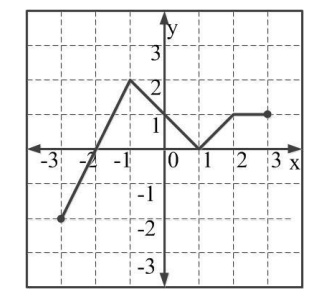
\includegraphics[width=0.5\textwidth]{figures/Q8.png}
\end{center}
\begin{enumerate}
    \item[(i)] \( y = 2x + 4 \) for \(-3 \leq x \leq -1\)
    \item[(ii)] \( y = |x - 1| \) for \(-1 \leq x \leq 2\)
    \item[(iii)] \( y = ||x| - 1| \) for \(-1 \leq x \leq 2\)
    \item[(iv)] \( y = 1 \) for \( 2 \leq x \leq 3 \)
\end{enumerate}

\begin{enumerate}
    \item[(A)] (i), (ii) and (iii) only.
    \item[(B)] (i), (ii) and (iv) only.
    \item[(C)] (i) and (iv) only.
    \item[(D)] (ii) and (iv) only.
\end{enumerate}
\vspace{0.5cm}

\questionb{Consider a sequence of numbers \( a_1, a_2, a_3, \cdots, a_n \) where \( a_n = \frac{1}{n} - \frac{1}{n+2} \), for each integer \( n > 0 \). What is the sum of the first 50 terms?}{9}
\begin{enumerate}
    \item[(A)] \( \left( 1 + \frac{1}{2} \right) - \frac{1}{50} \)
    \item[(B)] \( \left( 1 + \frac{1}{2} \right) + \frac{1}{50} \)
    \item[(C)] \( \left( 1 + \frac{1}{2} \right) - \left( \frac{1}{51} + \frac{1}{52} \right) \)
    \item[(D)] \( 1 - \left( \frac{1}{51} + \frac{1}{52} \right) \)
\end{enumerate}
\vspace{0.5cm}

\questionb{Each of the letters arranged as below represents a unique integer from 1 to 9. The letters are positioned in the figure such that (A × B × C), (B × G × E) and (D × E × F) are equal. Which integer among the following choices cannot be represented by the letters A, B, C, D, E, F or G?}{10}

\begin{tabular}{|c|c|c}
\hline
A &  &D \\
\hline
B & G & E \\
\hline
C &  &F \\
\hline
\end{tabular}

\begin{enumerate}
    \item[(A)] 4  
    \item[(B)] 5  
    \item[(C)] 6  
    \item[(D)] 9  
\end{enumerate}
\vspace{0.5cm}

% Technical Section
\section*{Technical Section}

\questiona{Which one of the following matrices is singular?}{1}
\begin{enumerate}
    \item[(A)] $\begin{bmatrix} 2 & 5 \\ 1 & 3 \end{bmatrix}$
    \item[(B)] $\begin{bmatrix} 3 & 2 \\ 2 & 3 \end{bmatrix}$
    \item[(C)] $\begin{bmatrix} 2 & 4 \\ 3 & 6 \end{bmatrix}$
    \item[(D)] $\begin{bmatrix} 4 & 3 \\ 6 & 2 \end{bmatrix}$
\end{enumerate}
\vspace{0.5cm}

\questiona{For the given orthogonal matrix Q,
\[ Q = \begin{bmatrix} 3/7 & 2/7 & 6/7 \\ -6/7 & 3/7 & 2/7 \\ 2/7 & 6/7 & -3/7 \end{bmatrix} \]
The inverse is}{2}
\begin{enumerate}
    \item[(A)] $\begin{bmatrix} 3/7 & 2/7 & 6/7 \\ -6/7 & 3/7 & 2/7 \\ 2/7 & 6/7 & -3/7 \end{bmatrix}$
    \item[(B)] $\begin{bmatrix} -3/7 & -2/7 & -6/7 \\ 6/7 & -3/7 & -2/7 \\ -2/7 & -6/7 & 3/7 \end{bmatrix}$
    \item[(C)] $\begin{bmatrix} 3/7 & -6/7 & 2/7 \\ 2/7 & 3/7 & 6/7 \\ 6/7 & 2/7 & -3/7 \end{bmatrix}$
    \item[(D)] $\begin{bmatrix} -3/7 & 6/7 & -2/7 \\ -2/7 & -3/7 & -6/7 \\ -6/7 & -2/7 & 3/7 \end{bmatrix}$
\end{enumerate}
\vspace{0.5cm}

\questiona{At the point \( x = 0 \), the function \( f(x) = x^3 \) has}{3}
\begin{enumerate}
    \item[(A)] local maximum
    \item[(B)] local minimum
    \item[(C)] both local maximum and minimum
    \item[(D)] neither local maximum nor local minimum
\end{enumerate}
\vspace{0.5cm}

\questiona{A column of height \( h \) with a rectangular cross-section of size \( a \times 2a \) has a buckling load of \( P \). If the cross-section is changed to \( 0.5a \times 3a \) and its height changed to \( 1.5h \), the buckling load of the redesigned column will be}{4}
\begin{enumerate}
    \item[(A)] \( P/12 \)
    \item[(B)] \( P/4 \)
    \item[(C)] \( P/2 \)
    \item[(D)] \( 3P/4 \)
\end{enumerate}
\vspace{0.5cm}

\questiona{A steel column of ISHB 350 @72.4 kg/m is subjected to a factored axial compressive load of 2000 kN. The load is transferred to a concrete pedestal of grade M20 through a square base plate. Consider bearing strength of concrete as \( 0.45f_{ck} \), where \( f_{ck} \) is the characteristic strength of concrete. Using limit state method and neglecting the self weight of base plate and steel column, the length of a side of the base plate to be provided is}{5}
\begin{enumerate}
    \item[(A)] 39 cm
    \item[(B)] 42 cm
    \item[(C)] 45 cm
    \item[(D)] 48 cm
\end{enumerate}
\vspace{0.5cm}

\questiona{The Le Chatelier apparatus is used to determine}{6}
\begin{enumerate}
    \item[(A)] compressive strength of cement
    \item[(B)] fineness of cement
    \item[(C)] setting time of cement
    \item[(D)] soundness of cement
\end{enumerate}
\vspace{0.5cm}

\questiona{The deformation in concrete due to sustained loading is}{7}
\begin{enumerate}
    \item[(A)] creep
    \item[(B)] hydration
    \item[(C)] segregation
    \item[(D)] shrinkage
\end{enumerate}
\vspace{0.5cm}

\questiona{A solid circular beam with radius of 0.25 m and length of 2 m is subjected to a twisting moment of 20 kNm about the z-axis at the free end, which is the only load acting as shown in the figure. The shear stress component \( \tau_{xy} \) at Point 'M' in the cross-section of the beam at a distance of 1 m from the fixed end is}{8}
\begin{center}
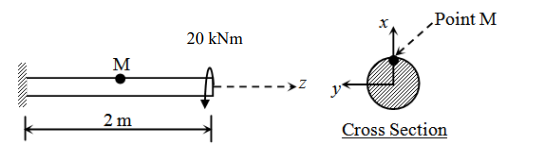
\includegraphics[width=0.5\textwidth]{figures/Q8a.png}
\end{center}
\begin{enumerate}
    \item[(A)] 0.0 MPa
    \item[(B)] 0.51 MPa
    \item[(C)] 0.815 MPa
    \item[(D)] 2.0 MPa
\end{enumerate}
\vspace{0.5cm}

\questiona{Two rectangular under-reinforced concrete beam sections X and Y are similar in all aspects except that the longitudinal compression reinforcement in section Y is 10\% more. Which one of the following is the correct statement?}{9}
\begin{enumerate}
    \item[(A)] Section X has less flexural strength and is less ductile than section Y
    \item[(B)] Section X has less flexural strength but is more ductile than section Y
    \item[(C)] Sections X and Y have equal flexural strength but different ductility
    \item[(D)] Sections X and Y have equal flexural strength and ductility
\end{enumerate}
\vspace{0.5cm}

\questiona{The percent reduction in the bearing capacity of a strip footing resting on sand under flooding condition (water level at the base of the footing) when compared to the situation where the water level is at a depth much greater than the width of footing, is approximately}{10}
\begin{enumerate}
    \item[(A)] 0
    \item[(B)] 25
    \item[(C)] 50
    \item[(D)] 100
\end{enumerate}
\vspace{0.5cm}

\questiona{The width of a square footing and the diameter of a circular footing are equal. If both the footings are placed on the surface of sandy soil, the ratio of the ultimate bearing capacity of circular footing to that of square footing will be}{11}
\begin{enumerate}
    \item[(A)] 4/3
    \item[(B)] 1
    \item[(C)] 3/4
    \item[(D)] 2/3
\end{enumerate}
\vspace{0.5cm}

\questiona{Bernoulli's equation is applicable for}{12}
\begin{enumerate}
    \item[(A)] viscous and compressible fluid flow
    \item[(B)] inviscid and compressible fluid flow
    \item[(C)] inviscid and incompressible fluid flow
    \item[(D)] viscous and incompressible fluid flow
\end{enumerate}
\vspace{0.5cm}

\questiona{There are 20,000 vehicles operating in a city with an average annual travel of 12,000 km per vehicle. The NOx emission rate is 2.0 g/km per vehicle. The total annual release of NOx will be}{13}
\begin{enumerate}
    \item[(A)] 4,80,000 kg
    \item[(B)] 4,800 kg
    \item[(C)] 480 kg
    \item[(D)] 48 kg
\end{enumerate}
\vspace{0.5cm}

\questiona{A bitumen sample has been graded as VG30 as per IS : 73-2013. The '30' in the grade means that}{14}
\begin{enumerate}
    \item[(A)] penetration of bitumen at 25°C is between 20 and 40
    \item[(B)] viscosity of bitumen at 60°C is between 2400 and 3600 Poise
    \item[(C)] ductility of bitumen at 27°C is more than 30 cm
    \item[(D)] elastic recovery of bitumen at 15°C is more than 30\%
\end{enumerate}
\vspace{0.5cm}

\questiona{The speed-density relationship for a road section is shown in the figure.}{15}
\begin{center}
\includegraphics[width=0.5\textwidth]{figures/q15}
\end{center}
The shape of the flow-density relationship is
\begin{enumerate}
    \item[(A)] piecewise linear
    \item[(B)] parabolic
    \item[(C)] initially linear then parabolic
    \item[(D)] initially parabolic then linear
\end{enumerate}
\vspace{0.5cm}

\questiona{A well-designed signalized intersection is one in which the}{16}
\begin{enumerate}
    \item[(A)] crossing conflicts are increased
    \item[(B)] total delay is minimized
    \item[(C)] cycle time is equal to the sum of red and green times in all phases
    \item[(D)] cycle time is equal to the sum of red and yellow times in all phases
\end{enumerate}
\vspace{0.5cm}

\questiona{A flow field is given by \( u = y^2 \), \( v = -xy \), \( w = 0 \). Value of the z-component of the angular velocity (in radians per unit time, up to two decimal places) at the point \((0, -1, 1)\) is \_\_\_\_\_}{17}
\vspace{0.5cm}

\questiona{The frequency distribution of the compressive strength of 20 concrete cube specimens is given in the table.}{18}

\begin{tabular}{|c|c|}
\hline
\( f \) (MPa) & Number of specimens \\
\hline
23 & 4 \\
28 & 2 \\
22.5 & 5 \\
31 & 5 \\
29 & 4 \\
\hline
\end{tabular}

If \( \mu \) is the mean strength and \( \sigma \) is the standard deviation, the number of specimens (out of 20) with compressive strength less than \( \mu - 3\sigma \) is \_\_\_\_\_
\vspace{0.5cm}

\questiona{In a fillet weld, the direct shear stress and bending tensile stress are 50 MPa and 150 MPa, respectively. As per IS 800: 2007, the equivalent stress (in MPa, up to two decimal places) will be \_\_\_\_\_}{19}
\vspace{0.5cm}

\questiona{In a shrinkage limit test, the volume and mass of a dry soil pat are found to be 50 cm\(^3\) and 88 g, respectively. The specific gravity of the soil solids is 2.71 and the density of water is 1 g/cc. The shrinkage limit (in \%, up to two decimal places) is \_\_\_\_\_}{20}
\vspace{0.5cm}

\questiona{A core cutter of 130 mm height has inner and outer diameters of 100 mm and 106 mm, respectively. The area ratio of the core cutter (in \%, up to two decimal places) is \_\_\_\_\_}{21}
\vspace{0.5cm}

\questiona{A 1:50 model of a spillway is to be tested in the laboratory. The discharge in the prototype spillway is 1000 m\(^3\)/s. The corresponding discharge (in m\(^3\)/s, up to two decimal places) to be maintained in the model, neglecting variation in acceleration due to gravity, is \_\_\_\_\_}{22}
\vspace{0.5cm}

\questiona{A 10 m wide rectangular channel carries a discharge of 20 m\(^3\)/s under critical condition. Using \( g = 9.81 \, \text{m/s}^2 \), the specific energy (in m, up to two decimal places) is \_\_\_\_\_}{23}
\vspace{0.5cm}

\questiona{For routing of flood in a given channel using the Muskingum method, two of the routing coefficients are estimated as \( C_0 = -0.25 \) and \( C_1 = 0.55 \). The value of the third coefficient \( C_2 \) would be \_\_\_\_\_}{24}
\vspace{0.5cm}

\questiona{A city generates \( 40 \times 10^6 \) kg of municipal solid waste (MSW) per year, out of which only 10\% is recovered/recycled and the rest goes to landfill. The landfill has a single lift of 3 m height and is compacted to a density of 550 kg/m\(^3\). If 80\% of the landfill is assumed to be MSW, the landfill area (in m\(^2\), up to one decimal place) required would be \_\_\_\_\_}{25}
\vspace{0.5cm}

\questionb{The value of the integral \( \int_{0}^{\pi} x \cos^{2} x \, dx \) is}{26}
\begin{enumerate}
    \item[(A)] \( \pi^{2}/8 \)
    \item[(B)] \( \pi^{2}/4 \)
    \item[(C)] \( \pi^{2}/2 \)
    \item[(D)] \( \pi^{2} \)
\end{enumerate}
\vspace{0.5cm}

\questionb{A cantilever beam of length 2 m with a square section of side length 0.1 m is loaded vertically at the free end. The vertical displacement at the free end is 5 mm. The beam is made of steel with Young's modulus of \( 2.0 \times 10^{11} \) N/m\(^2\). The maximum bending stress at the fixed end of the cantilever is}{27}
\begin{enumerate}
    \item[(A)] 20.0 MPa
    \item[(B)] 37.5 MPa
    \item[(C)] 60.0 MPa
    \item[(D)] 75.0 MPa
\end{enumerate}
\vspace{0.5cm}

\questionb{A cylinder of radius 250 mm and weight, \( W = 10 \) kN is rolled up an obstacle of height 50 mm by applying a horizontal force P at its centre as shown in the figure.}{28}
\begin{center}
\includegraphics[width=0.5\textwidth]{figures/q28}
\end{center}
All interfaces are assumed frictionless. The minimum value of P is
\begin{enumerate}
    \item[(A)] 4.5 kN
    \item[(B)] 5.0 kN
    \item[(C)] 6.0 kN
    \item[(D)] 7.5 kN
\end{enumerate}
\vspace{0.5cm}

\questionb{A plate in equilibrium is subjected to uniform stresses along its edges with magnitude \( \sigma_{xx} = 30 \) MPa and \( \sigma_{yy} = 50 \) MPa as shown in the figure.}{29}
\begin{center}
\includegraphics[width=0.5\textwidth]{figures/q29}
\end{center}
The Young's modulus of the material is \( 2 \times 10^{11} \) N/m\(^2\) and the Poisson's ratio is 0.3. If \( \sigma_{zz} \) is negligibly small and assumed to be zero, then the strain \( \varepsilon_{zz} \) is
\begin{enumerate}
    \item[(A)] \( -120 \times 10^{-6} \)
    \item[(B)] \( -60 \times 10^{-6} \)
    \item[(C)] 0.0
    \item[(D)] \( 120 \times 10^{-6} \)
\end{enumerate}
\vspace{0.5cm}

\questionb{The figure shows a simply supported beam PQ of uniform flexural rigidity \( EI \) carrying two moments \( M \) and \( 2M \).}{30}
\begin{center}
\includegraphics[width=0.5\textwidth]{figures/q30}
\end{center}
The slope at P will be
\begin{enumerate}
    \item[(A)] 0
    \item[(B)] \( ML/(9EI) \)
    \item[(C)] \( ML/(6EI) \)
    \item[(D)] \( ML/(3EI) \)
\end{enumerate}
\vspace{0.5cm}

\questionb{A 0.5 m × 0.5 m square concrete pile is to be driven in a homogeneous clayey soil having undrained shear strength, \( c_u = 50 \) kPa and unit weight, \( \gamma = 18.0 \) kN/m\(^3\). The design capacity of the pile is 500 kN. The adhesion factor \( \alpha \) is given as 0.75. The length of the pile required for the above design load with a factor of safety of 2.0 is}{31}
\begin{enumerate}
    \item[(A)] 5.2 m
    \item[(B)] 5.8 m
    \item[(C)] 11.8 m
    \item[(D)] 12.5 m
\end{enumerate}
\vspace{0.5cm}

\questionb{A closed tank contains 0.5 m thick layer of mercury (specific gravity = 13.6) at the bottom. A 2.0 m thick layer of water lies above the mercury layer. A 3.0 m thick layer of oil (specific gravity = 0.6) lies above the water layer. The space above the oil layer contains air under pressure. The gauge pressure at the bottom of the tank is 196.2 kN/m\(^2\). The density of water is 1000 kg/m\(^3\) and the acceleration due to gravity is 9.81 m/s\(^2\). The value of pressure in the air space is}{32}
\begin{enumerate}
    \item[(A)] 92.214 kN/m\(^2\)
    \item[(B)] 95.644 kN/m\(^2\)
    \item[(C)] 98.922 kN/m\(^2\)
    \item[(D)] 99.321 kN/m\(^2\)
\end{enumerate}
\vspace{0.5cm}

\questionb{A rapid sand filter comprising a number of filter beds is required to produce 99 MLD of potable water. Consider water loss during backwashing as 5\%, rate of filtration as 6.0 m/h and length to width ratio of filter bed as 1.35. The width of each filter bed is to be kept equal to 5.2 m. One additional filter bed is to be provided to take care of break-down, repair and maintenance. The total number of filter beds required will be}{33}
\begin{enumerate}
    \item[(A)] 19
    \item[(B)] 20
    \item[(C)] 21
    \item[(D)] 22
\end{enumerate}
\vspace{0.5cm}

\questionb{A priority intersection has a single-lane one-way traffic road crossing an undivided two-lane two-way traffic road. The traffic stream speed on the single-lane road is 20 kmph and the speed on the two-lane road is 50 kmph. The perception-reaction time is 2.5 s, coefficient of longitudinal friction is 0.38 and acceleration due to gravity is 9.81 m/s\(^2\). A clear sight triangle has to be ensured at this intersection. The minimum lengths of the sides of the sight triangle along the two-lane road and the single-lane road, respectively will be}{34}
\begin{enumerate}
    \item[(A)] 50 m and 20 m
    \item[(B)] 61 m and 18 m
    \item[(C)] 111 m and 15 m
    \item[(D)] 122 m and 36 m
\end{enumerate}
\vspace{0.5cm}

\questionb{The following details refer to a closed traverse:}{35}

\begin{tabular}{|c|c|c|c|c|}
\hline
Line & Northing (m) & Southing (m) & Easting (m) & Westing (m) \\
\hline
PQ & --- & 437 & 173 & --- \\
QR & 101 & --- & 558 & --- \\
RS & 419 & --- & --- & 96 \\
SP & --- & 83 & --- & 634 \\
\hline
\end{tabular}

The length and direction (whole circle bearing) of closure, respectively are
\begin{enumerate}
    \item[(A)] 1 m and 90°
    \item[(B)] 2 m and 90°
    \item[(C)] 1 m and 270°
    \item[(D)] 2 m and 270°
\end{enumerate}
\vspace{0.5cm}

\questionb{A square area (on the surface of the earth) with side 100 m and uniform height, appears as 1 cm\(^2\) on a vertical aerial photograph. The topographic map shows that a contour of 650 m passes through the area. If focal length of the camera lens is 150 mm, the height from which the aerial photograph was taken, is}{36}
\begin{enumerate}
    \item[(A)] 800 m
    \item[(B)] 1500 m
    \item[(C)] 2150 m
    \item[(D)] 3150 m
\end{enumerate}
\vspace{0.5cm}

\questionb{The solution at \( x = 1 \), \( t = 1 \) of the partial differential equation \(\frac{\partial^2 u}{\partial x^2} = 25 \frac{\partial^2 u}{\partial t^2}\) subject to initial conditions of \( u(0) = 3x \) and \(\frac{\partial u}{\partial t}(0) = 3 \) is}{37}
\begin{enumerate}
    \item[(A)] 1
    \item[(B)] 2
    \item[(C)] 4
    \item[(D)] 6
\end{enumerate}
\vspace{0.5cm}

\questionb{The solution (up to three decimal places) at \( x = 1 \) of the differential equation \(\frac{d^2 y}{dx^2} + 2 \frac{dy}{dx} + y = 0 \) subject to boundary conditions \( y(0) = 1 \) and \(\frac{dy}{dx}(0) = -1 \) is \_\_\_\_\_}{38}
\vspace{0.5cm}

\questionb{Variation of water depth (\( y \)) in a gradually varied open channel flow is given by the first order differential equation}{39}

\[ \frac{dy}{dx} = \frac{1 - e^{-\frac{10}{3} \ln(y)}}{250 - 45e^{-3 \ln(y)}} \]

Given initial condition: \( y(x = 0) = 0.8 \) m. The depth (in m, up to three decimal places) of flow at a downstream section at \( x = 1 \) m from one calculation step of Single Step Euler Method is \_\_\_\_\_
\vspace{0.5cm}

\questionb{An RCC short column (with lateral ties) of rectangular cross section of 250 mm × 300 mm is reinforced with four numbers of 16 mm diameter longitudinal bars. The grades of steel and concrete are Fe415 and M20, respectively. Neglect eccentricity effect. Considering limit state of collapse in compression (IS 456 : 2000), the axial load carrying capacity of the column (in kN, up to one decimal place), is \_\_\_\_\_}{40}
\vspace{0.5cm}

\questionb{An RCC beam of rectangular cross section has factored shear of 200 kN at its critical section. Its width \( b \) is 250 mm and effective depth \( d \) is 350 mm. Assume design shear strength \( \tau_c \) of concrete as 0.62 N/mm\(^2\) and maximum allowable shear stress \( \tau_{c,max} \) in concrete as 2.8 N/mm\(^2\). If two legged 10 mm diameter vertical stirrups of Fe250 grade steel are used, then the required spacing (in cm, up to one decimal place) as per limit state method will be \_\_\_\_\_}{41}
\vspace{0.5cm}

\questionb{The dimensions of a symmetrical welded I-section are shown in the figure.}{42}
\begin{center}
\includegraphics[width=0.5\textwidth]{figures/q42}
\end{center}
(All dimensions are in mm)

The plastic section modulus about the weaker axis (in cm\(^3\), up to one decimal place) is \_\_\_\_\_
\vspace{0.5cm}

\questionb{Consider the deformable pin-jointed truss with loading, geometry and section properties as shown in the figure.}{43}
\begin{center}
\includegraphics[width=0.5\textwidth]{figures/q43}
\end{center}
Given that \( E = 2 \times 10^{11} \) N/m\(^2\), \( A = 10 \) mm\(^2\), \( L = 1 \) m and \( P = 1 \) kN. The horizontal displacement of Joint C (in mm, up to one decimal place) is \_\_\_\_\_
\vspace{0.5cm}

\questionb{At a construction site, a contractor plans to make an excavation as shown in the figure.}{44}
\begin{center}
\includegraphics[width=0.5\textwidth]{figures/q44}
\end{center}
The water level in the adjacent river is at an elevation of +20.0 m. Unit weight of water is 10 kN/m\(^3\). The factor of safety (up to two decimal places) against sand boiling for the proposed excavation is \_\_\_\_\_
\vspace{0.5cm}

\questionb{A conventional drained triaxial compression test was conducted on a normally consolidated clay sample under an effective confining pressure of 200 kPa. The deviator stress at failure was found to be 400 kPa. An identical specimen of the same clay sample is isotropically consolidated to a confining pressure of 200 kPa and subjected to standard undrained triaxial compression test. If the deviator stress at failure is 150 kPa, the pore pressure developed (in kPa, up to one decimal place) is \_\_\_\_\_}{45}
\vspace{0.5cm}

\questionb{The void ratio of a soil is 0.55 at an effective normal stress of 140 kPa. The compression index of the soil is 0.25. In order to reduce the void ratio to 0.4, an increase in the magnitude of effective normal stress (in kPa, up to one decimal place) should be \_\_\_\_\_}{46}
\vspace{0.5cm}

\questionb{A rigid smooth retaining wall of height 7 m with vertical backface retains saturated clay as backfill. The saturated unit weight and undrained cohesion of the backfill are 17.2 kN/m\(^3\) and 20 kPa, respectively. The difference in the active lateral forces on the wall (in kN per meter length of wall, up to two decimal places), before and after the occurrence of tension cracks is \_\_\_\_\_}{47}
\vspace{0.5cm}

\questionb{Rainfall depth over a watershed is monitored through six number of well distributed rain gauges. Gauged data are given below}{48}

\begin{tabular}{|c|c|c|c|c|c|c|}
\hline
Rain Gauge Number & 1 & 2 & 3 & 4 & 5 & 6 \\
\hline
Rainfall Depth (mm) & 470 & 465 & 435 & 525 & 480 & 510 \\
Area of Thiessen Polygon (×10\(^4\) m\(^2\)) & 95 & 100 & 98 & 80 & 85 & 92 \\
\hline
\end{tabular}

The Thiessen mean value (in mm, up to one decimal place) of the rainfall is \_\_\_\_\_
\vspace{0.5cm}

\questionb{The infiltration rate \( f \) in a basin under ponding condition is given by \( f = 30 + 10e^{-2t} \), where, \( f \) is in mm/h and \( t \) is time in hour. Total depth of infiltration (in mm, up to one decimal place) during the last 20 minutes of a storm of 30 minutes duration is \_\_\_\_\_}{49}
\vspace{0.5cm}

\questionb{In a laboratory, a flow experiment is performed over a hydraulic structure. The measured values of discharge and velocity are 0.05 m\(^3\)/s and 0.25 m/s, respectively. If the full scale structure (30 times bigger) is subjected to a discharge of 270 m\(^3\)/s, then the time scale (model to full scale) value (up to two decimal places) is \_\_\_\_\_}{50}
\vspace{0.5cm}

\questionb{A water sample analysis data is given below.}{51}

\begin{tabular}{|c|c|c|}
\hline
Ion & Concentration, mg/L & Atomic Weight \\
\hline
Ca\(^{2+}\) & 60 & 40 \\
Mg\(^{2+}\) & 30 & 24.31 \\
HCO\(_3^-\) & 400 & 61 \\
\hline
\end{tabular}

The carbonate hardness (expressed as mg/L of CaCO\(_3\), up to one decimal place) for the water sample is \_\_\_\_\_
\vspace{0.5cm}

\questionb{The ultimate BOD \( L_0 \) of a wastewater sample is estimated as 87\% of COD. The COD of this wastewater is 300 mg/L. Considering first order BOD reaction rate constant k (use natural log) = 0.23 per day and temperature coefficient $\theta$ = 1.047, the BOD value (in mg/L, up to one decimal place) after three days of incubation at 27°C for this wastewater will be \_\_\_\_\_}{52}
\vspace{0.5cm}

\questionb{A waste activated sludge (WAS) is to be blended with green waste (GW). The carbon (C) and nitrogen (N) contents, per kg of WAS and GW, on dry basis are given in the table.}{53}

\begin{tabular}{|c|c|c|}
\hline
Parameter & WAS & GW \\
\hline
Carbon (g) & 54 & 360 \\
Nitrogen (g) & 10 & 6 \\
\hline
\end{tabular}

The ratio of WAS to GW required (up to two decimal places) to achieve a blended C:N ratio of 20:1 on dry basis is \_\_\_\_\_
\vspace{0.5cm}

\questionb{Given the following data: design life n = 15 years, lane distribution factor D = 0.75, annual rate of growth of commercial vehicles r = 6\%, vehicle damage factor F = 4 and initial traffic in the year of completion of construction = 3000 Commercial Vehicles Per Day (CVPD). As per IRC:37-2012, the design traffic in terms of cumulative number of standard axles (in million standard axles, up to two decimal places) is \_\_\_\_\_}{54}
\vspace{0.5cm}

\questionb{An aircraft approaches the threshold of a runway strip at a speed of 200 km/h. The pilot decelerates the aircraft at a rate of 1.697 m/s\(^2\) and takes 18 s to exit the runway strip. If the deceleration after exiting the runway is 1 m/s\(^2\), then the distance (in m, up to one decimal place) of the gate position from the location of exit on the runway is \_\_\_\_\_}{55}
\vspace{1 cm}

\begin{center}
\textbf{END OF THE QUESTION PAPER}
\rule{\textwidth}{0.5pt}
\end{center}
\end{document}

